\chapter{Re\c{t}elele neuronale}

\section{Neuronul}

Re\c{t}elele Neuronale au pornit de la ideea de a crea un model matematic care s\u{a} imite structura \c{s}i comportamentul unui creier uman.
\par
Creierul este compus din mai multe unit\u{a}\c{t}i numi\c{t}i neuroni, care comunic\u{a} \^{i}ntre ei prin sinapse, se aproximeaz\u{a} faptul c\u{a} creierul uman are aproximativ 86 de miliarde de neuroni \c{s}i 10^{14} - 10^{15}  sinapse.


\includegraphics[width=300]{neuron_small.png}

Fiecare neuron prime\c{s}te impulsuri prin dedridele sale de la al\c{t}i neuroni \c{s}i produce impulsuri prin axon pe care il transmite mai departe la al\c{t}i neuroni prin sinapse.

\par

Acest model biologic a incercat sa fie imitat de c\u{a}tre Warren McCulloch \c{s}i Walter Pitts \^{i}n anul 1943, astfle \^{i}ncat ace\c{s}tia au creat un model matematic care s\u{a} semene c\^{a}t mai mult cu varianta biologic\u{a}. \^{I}n modelul matematic propus de ace\c{s}tia datele de intrare primite prin dendrive ( s\u{a} le not\u{a}m cu \textbf{\textit{x}} ) sunt multiplicate cu ni\c{s}te \^{i}nt\u{a}riri ( s\u{a} le not\u{a}m cu \textbf{\textit{W}} ) pentru a se imita transferul facut prin sinapse \^{i}ntre axonul neuronului care transmite datle \c{s}i dendrivele neuronului care prime\c{s}te datele. Corpul neuronului a devenit un sumator care \^{i}nsumeaza produsul primit de la dendrive, astfel c\u{a} acesta se poate definii prin urm\u{a}toarea formul\u{a}  $$ \sum_{i=1}^{n} W_i x_i $$ unde \textbf{\textit{n}} reprezint\u{a} num\u{a}rul de dendrive. La aceast\u{a} formul\u{a} se mai insumeaz\u{a} un \textit{biases} ( s\u{a} \^{i}l not\u{a}m cu \textbf{\textit{b}} ) pentru a reprezenta caracteristicile neliniare ale neuronului. Cu aceast\u{a} nou\u{a} \^{i}nsumare formula va devenii $$ \sum_{i=1}^{n} W_i x_i + b $$
Dac\u{a} rezultatul ob\c{t}inut este mai mare dec\^{a}t un prag acesta va trece mai departe prin axon spre al\c{t}i neuroni. S\u{a} definim acest efect printr-o func\c{t}ie \textbf{\textit{f}} pe care o vom numii \textit{func\c{t}ie de activare} care stabile\c{s}te dac\u{a} un semnal trece mai departe sau nu, vom descrie mai pe larg aceast\u{a} func\c{t}ie in capitolele de mai jos, astfel c\u{a} modelul matematic a neuronului se poate rezuma la urm\u{a}toarea formul\u{a} 
$$f( \sum_{i=1}^{n} W_i x_i + b ) $$

\par

Trebuie precizat faptul c\u{a} modelul matematic al neuronului prezentat mai sus nici mac\u{a} nu se apropie de adevaratul comportament al unui neuron, acesta din urm\u{a} av\^{a}nd \^{i}n creierul uman un rol mult prea complex pentru a putea fi exprimat printr-o simpl\u{a} func\c{t}ie. 


\section{Fun\c{t}ia de activare}

A\c{s}a cum am specificat \c{s}i mai sus, o re\c{t}ea neuronala are nevoie de o fun\c{t}ie de activare care s\u{a} decid\u{a} dac\u{a} datele pot trece mai departe la urmatorii neuroni sau nu. De-a lungu istoriei s-au folosit mai multe tipuri de fun\c{t}ii de activare la re\c{t}elele neuronale, \^{i}nsa cea care d\u{a} cel mai bun randament at\^{a}t la timpul de antrenare c\^{a}t \c{s}i la acurate\c{t}ea final\u{a} este func\c{t}ia de activare ReLU (Rectified Linear Unit).

\subsection{Rectified Linear Unit}

Rectified Linear Unit, sau mai pe scurt ReLU, este la ora actual\u{a} cea mai folosit\u{a} fun\c{t}ie de activare, ea av\^{a}nd urm\u{a}toarea formul\u{a}

\[ f(x) =
  \begin{cases}
    0       & \quad \text{dac\u{a} } x \leq 0\\
    x  & \quad \text{dac\u{a} } x > 0\\
  \end{cases}
\]

Cu alte cuvinte func\c{t}ia pur \c{s}i simplu nu las\u{a} s\u{a} treac\u{a} mai departe rezultatele negative in urma efectu\u{a}rii opera\c{t}iilor din corpul neuronului.

\section{Arhitectura unei re\c{t}ele neuronale}

Acum c\u{a} am aflat ce este un neuron \c{s}i cum este simulat acesta din punct de vedere matematic trebuie s\u{a} discut\u{a}m cum sunt structura\c{t}i ace\c{s}tia \^{i}ntr-o re\c{t}ea neuronal\u{a}, pentru c\u{a} o re\c{t}ea nuronal\u{a} este compus\u{a} din milioane sau chiar sute de milioane de neuroni iar structurarea acestora este foarte important\u{a}.

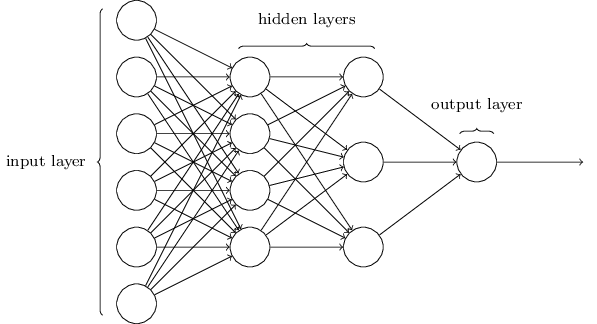
\includegraphics[width=300]{image10.png}

Re\c{t}elele neuronale sunt modelate ca o cole\c{t}ie de neuroni pe nivele, unde datele calculate de un nivel devin datele de intrare pentru urmatorul nivel de neuroni. Dupa cum se vede \c{s}i in imaginea de mai sus, neuronii afla\c{t}i pe acela\c{s}i nivel nu comunic\u{a} direct unii cu ceilal\c{t}i, comunicarea realiz\^{a}nduse doar cu nivelul inferior de neuroni \c{s}i cu nivelul superior de neuroni.
\par
Primul nivel al unei re\c{t}ele neuronale se nume\c{s}te nivelu input, deoarece acesta reprezint\u{a} doar date de intrare, iar ultimul nivel al unei re\c{t}ele neuronale se nume\c{s}te nivelul output, doarece acesta intoarce valoarea final\u{a}, nivelele dintre primul \c{s}i ultimul nivel se numesc nivelele ascunse ( hidden layers ).
\par
Re\c{t}elele neuronale, ca cea de mai sus, se numesc re\c{t}ele feedforward, deoarece outputul unui nivel merge tot timpul la urm\u{a}torul nivel, nu se intoarce niciodat\u{a} la un nivel anterior.
\par 
Pentru a se in\c{t}elege mai bine cum lucreaz\u{a} o re\c{t}ea neuronal\u{a} vom nota cu \textbf{\textit{x}} datele de intrare de la nivelul input, cu \textbf{\textit{h}} fiecare hidden layer, cu \textbf{\textit{W}} \^{i}ntaririle, cu \textbf{\textit{b}} bias-ul si cu \textbf{\textit{f}} func\c{t}ia de activare, astfle c\u{a} modelul de mai sus cu dou\u{a} niveluri hidden se poate exprima prin urm\u{a}torul algoritm:

$$h_1 = f( \sum_{i=1}^{n} W_1_i x_i + b_1 ) $$
$$h_2 = f( \sum_{i=1}^{n} W_2_i h_1_i + b_2 ) $$
$$out = f( \sum_{i=1}^{n} W_3_i h_2_i + b_3 ) $$

\par

Unul dintre motivele pentru care re\c{t}elele neuronale sunt organizate pe nivele este acela c\u{a} pe acest timp de structur\u{a} este mai u\c{s}or s\u{a} se efectueze opera\c{t}ii pe matrici, astfel inc\^{a}t sa nu mai fim nevoi\c{t}i s\u{a} facem multiplic\u{a}ri individuale. Spre exemplu, s\u{a} lu\u{a}m un \textbf{\textit{x}} de dimeniusne [10x10], $W_1, W_2 $ \c{s}i $W_3$ de dimensiune [5x10], [3x5], respectiv [1x3], iar $b_1, b_2 $ \c{s}i $b_3$ de dimensiune [5x1], [3x1] \c{s}i [1x1], atunci algoritmul de mai sus se poate rescrie in felul urmator: 

$$h_1 = f( W_1 x + b_1 ) $$
$$h_2 = f( W_2 h_1 + b_2 ) $$
$$out = f( W_3 h_2 + b_3 ) $$

unde $h_1$ este de dimensiune [5x10], $h_2$ de dimensiune [3x10], iar out de dimensiune [1x10]. Parametrii $W_1, W_2, W_3, b_1, b_2, b_3$ sunt paramterii pe care re\c{t}eaua neuronal\u{a} \^{i}i inva\c{t}\u{a} pentru a atinge o accurate\c{t}e c\^{a}t mai mare. Despre procesul de inv\u{a}\c{t}are a parametrilor \c{s}i despre cum trebuie s\u{a} \^{i}i set\u{a}m la inceput vom discuta \^{i}n capitolele ce urmeaz\u{a}.

\section{Initializarea parametrilor}

Am v\u{a}zut mai sus cum s\u{a} construim o re\c{t}ea neuronal\u{a}. \^{I}nainte ca s\u{a} discut\u{a}m descpre cum se antreneaz\u{a} o re\c{t}ea neuronal\u{a} trebuie s\u{a} discumta cum ini\c{t}ializ\u{a}m cele dou\u{a} tipuri de parametrii (\^{i}nt\u{a}ririle \c{s}i bias - urile). 

\subsection{Initializarea \^{i}nt\u{a}ririlor}

Av\^{a}nd in vedere c\u{a} nu \c{s}tiim valorile finale pe care o s\u{a} le aibe \^{i}nt\u{a}ririle la finalul procesului de antrenare a re\c{t}elei neuronale, deoarece aceste valori se actualizeaz\u{a} la fiecare pas de antrenare, va trebuii s\u{a} ini\c{t}ializ\u{a}m \^{i}nt\u{a}ririle astfle \^{i}nc\^{a}t o jum\u{a}tate din valori s\u{a} aibe valori negative iar cealalt\u{a} jum\u{a}tate valori pozitive, vom dorii valori unice pentru fiecare \^{i}ntarire pentru a acoperii o gam\u{a} c\^{a}t mai larg\u{a} de valori posibile pentru \^{i}nt\u{a}riri iar acestea s\u{a} fiu c\^{a}t mai aproape de valorea zero dar diferite de zero astfle \^{i}nc\^{a}t s\u{a} fiu mai u\c{s}or de actualizat.

\par

Pentru a \^{i}ndeplinii condi\c{t}iile de mai sus vom folosii o distribu\c{t}ie normal\u{a} cu media zero \c{s}i cu devia\c{t}ia standard $\frac{1}{\sqrt{n}}$ , unde n reprezint\u{a} numarul de variabile pe care \^{i}nt\u{a}rirea o are. Acest lucru asigur\u{a} faptul c\u{a} toate \^{i}nt\u{a}ririle din re\c{t}eaua neuronal\u{a} au la inceput aceea\c{s}i distribu\c{t}ie de numere, lucru care va facilita antrenarea mai rapid\u{a} a re\c{t}elei neuronale.

\par 

Dup\u{a} cum \c{s}tiim, varian\c{t}a reprezint\u{a} media patratic\u{a} a abaterilor in m\u{a}rime absolut\u{a} a valorilor inregistrare fat\u{a} de media aritmetic\u{a} care ne spune c\^{a}t de mare este r\u{a}sp\^{a}ndirea  acestui set. Mai precis, varian\c{t}a m\u{a}soar\u{a} c\^{a}t de apropiate sunt valorile setului de date de valoarea medie a acestuia.

$$Var = \frac{1}{n} \sum_{i=1}^{n} (x_i - m )^2 $$

\^{I}n formula de mai sus m reprezint\u{a} media aritmetic\u{a} iar $x_i$ valaorile date. \^{I}n cazul nostru dorim ca varian\c{t}a datelor de intrare sa nu se schimbe dup\u{a} ce iese din neuron \c{s}i se duce spre func\c{t}ia de activare pentru a nu altera datele foarte tare de la un nivel la altul. \^{I}n acest caz

$$Var(\sum_{i=1}^{n} W_i x_i) = \sum_{i=1}^{n} Var(W_i x_i) = $$
$$ = \sum_{i=1}^{n} [E(W_i)]^2 Var(x_i) + [E(x_i)]^2 Var(W_i) + Var(x_i) Var(W_i)$$

Presupunem c\u{a} setul de date \c{s}i \^{i}nt\u{a}ririle au media zero \c{s}i sunt distribuite identic, astfel c\u{a} formula de mai sus se transform\u{a} \^{i}n

$$\sum_{i=1}^{n} Var(x_i) Var(W_i) = (n Var(W)) Var(x)$$

care trebuie sa fie egal\u{a} cu varian\c{t}a datelor de intrare, asta \^{i}nseamn\u{a} c\u{a} 

$$n Var(W) = 1 \implies Var(W) =  \frac{1}{n} $$

\c{s}i \c{t}in\^{a}nd cont c\u{a} varian\c{t}a unei distribu\c{t}ii normale este p\u{a}tratul devia\c{t}iei standard, atunci rezult\u{a} c\u{a} devia\c{t}ia standard are valoarea $\frac{1}{\sqrt{n}}$ pentru distribu\c{t}ia normal\u{a} pe care o vom folosii pentru a alege valorile \^{i}nt\u{a}ririlor la ini\c{t}ializare.

\subsection{Initializarea bias}

Pentru bias-uri este comun de a le ini\c{t}ializa cu valorea zero sau cu o valoare foarte mic\u{a} apropiat\u{a} de zero, de exemplu 0.01. Din cauza faptului c\u{a} bias-ul nu joac\u{a} un rol a\c{s}a de important ca \^{i}nt\u{a}ririle \^{i}n re\c{t}eaua neuronal\u{a}, nu este de o importan\c{t}\u{a} foarte mare \^{i}n procesul de \^{i}nv\u{a}\c{t}are valoarea pe care o folosim la ini\c{t}ializarea lor, din acest motiv vom ini\c{t}ializa bias-ul cu valoarea zero.

\section{Procesul de antrenare}

Procesul de antrenare sau \^{i}nv\u{a}\c{t}are a unei re\c{t}ele neuronale const\u{a} din mai multe componente, prima component\u{a} se numeste func\c{t}ia de pierdere ( loss function \^{i}n englez\u{a} ) care penalizeaz\u{a} corectitudinea predic\c{t}iilor facute de c\u{a}tre re\c{t}eaua neuronal\u{a} fa\c{t}\u{a} de predic\c{t}iile corecte, a doua component\u{a} const\u{a} \^{i}n metode de prevenire a efectului de overfitting \^{i}n re\c{t}eaua neuronal\u{a}, a treia \c{s}i ultima component\u{a} este procesul de propagare \^{i}napoi care actualizeaz\u{a} \^{i}nt\u{a}ririle si bias-urile din re\c{t}eaua neuronal\u{a} astfel \^{i}nc\^{a}t urmatoarele predic\c{t}ii ale re\c{t}elei neuronale s\u{a} fiu mai aproape de adev\u{a}r. \^{I}n continuare vom definii mai detaliat cele trei componente.

\subsection{Func\c{t}ia de pierdere}

Func\c{t}ia de pierdere are rolul de a m\u{a}sura compatibilitatea dintre predic\c{t}iile f\u{a}cute de c\u{a}tre re\c{t}eaua neuronal\u{a} \c{s}i valorile adev\u{a}rate. Aceast\u{a} func\c{t}ie face media \^{i}ntre rezultatele ob\c{t}inute de c\u{a}tre fiecare predic\c{t}ie \^{i}n urma aplicarii unei func\c{t}ii de cost care m\u{a}soar\u{a} c\^{a}t de aproape este predic\c{t}ia de adev\u{a}r.

$$L = \frac{1}{N} \sum_i L_i $$

Exist\u{a} mai multe variante de func\c{t}ii de cost \^{i}ns\u{a} cea mai folosit\u{a} \c{s}i cea mai eficient\u{a} la ora actual\u{a} este func\c{t}ia Softmax, care are urm\u{a}toarea formul\u{a}

$$ L_i = - log \bigg(\frac{e^{f_y_i}}{\sum_j e^{f_j}}\bigg)$$

Unde $f_j$ reprezint\u{a} valoarea preconizat\u{a} de re\c{t}eaua neuronal\u{a} la pozi\c{t}ia j, iar $f_y_i$ reprzint\u{a} valorea preconizat\u{a} pentru valorea adevarat\u{a}.

\par

Pentru a se \^{i}n\c{t}elege mai bine cum func\c{t}ioneaz\u{a} func\c{t}ia Softmax o s\u{a} d\u{a}m un mic exemplu.